%斜坡模型受力分析图

\documentclass[11pt,tikz,border=3.14mm]{standalone}
\usepackage{pgfplots}
\pgfplotsset{compat=1.17}
\usetikzlibrary{calc}

\usepackage{mathptmx}
\usepackage{xcolor}
\definecolor{r1}{HTML}{FF8674}
\definecolor{b1}{HTML}{17ABDD}
\definecolor{p1}{HTML}{D4B6D6}
\definecolor{g1}{HTML}{70E2CB}
\definecolor{o1}{HTML}{DFA743}

\begin{document}

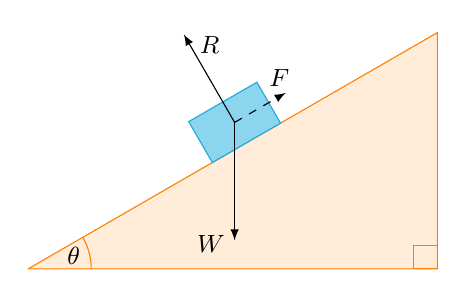
\begin{tikzpicture} [font = \small]
% triangle:
\draw [draw = orange, fill = orange!15] (0,0) coordinate (O) -- (30:6)
	coordinate [pos=.45] (M) |- coordinate (B) (O);

% angles:
\draw [draw = orange] (O) ++(.8,0) arc (0:30:0.8) 
	node [pos=.4, left] {$\theta$};
\draw [draw = orange] (B) rectangle ++(-0.3,0.3);



\begin{scope} [-latex,rotate=30]
% Object (rectangle)
\draw [fill = b1!50,
	draw = b1] (M) rectangle ++ (1,.6);

\coordinate (MM) at ($(M)+(0.5,0.3)$);
% Weight Force and its projections
%\draw [dashed] (M) ++ (.5,.3) coordinate (MM) -- ++ (0,-1.29)	node [very near end, right] {$mg\cos{\theta}$};

%\draw [dashed] (MM) -- ++ (-0.75,0) node [very near end, left] {$mg\sin{\theta}$};

\draw (MM) -- ++ (-30-90:1.5)
	node [very near end,below left ] {$W$};

% Normal Force
\draw (MM) -- ++ (0,1.29)
node [very near end, right] {$R$};

% Frictional Force
\draw[dashed] (MM) -- ++ (0.75,0)
	node [very near end, above] {$F$};

\end{scope}
\end{tikzpicture} 

\end{document}